\documentclass[11pt]{report}
\usepackage{import}
\usepackage{preamble}


\begin{document}

%%%%%%%%%%%%%%%%%%%%%%%%%%%%
%%% Cambiar 'Figura' por 'Imagen'
\renewcommand{\figurename}{Imagen}
\renewcommand{\listfigurename}{Lista de Imágenes}

%%%%%%%%%%%%%%%%%%%%%%%%%%%%
%%%% PORTADA
%%%%%%%%%%%%%%%%%%%%%%%%%%%%

\thispagestyle{empty}
\begin{titlepage}
    \hspace{-1.5cm}
	
\includegraphics[width=40mm]{img/LogoETSIIT.png}
	
\includegraphics[width=40mm]{img/LogoFacultadCiencias.jpeg}
	\hfill
	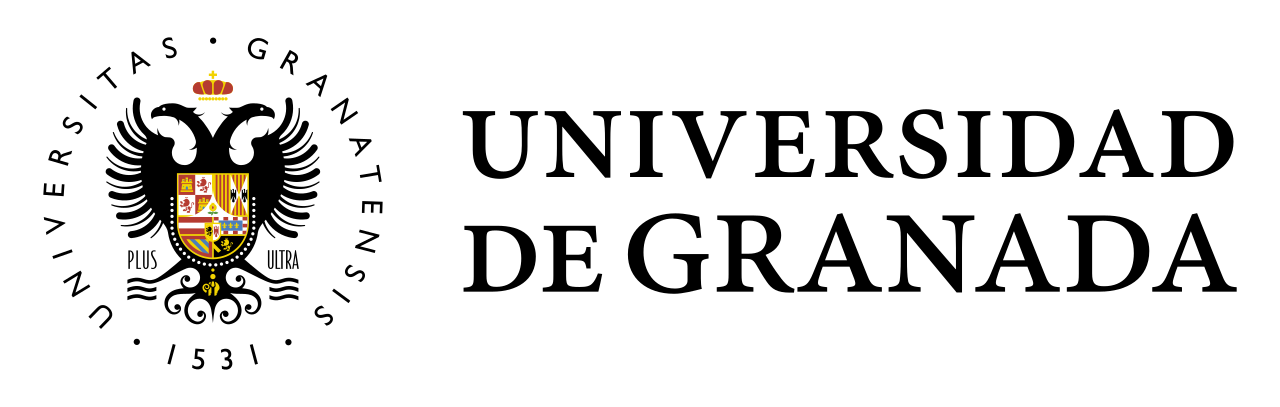
\includegraphics[width=50mm]{img/LogoUGR.png}
	
	\noindent\begin{small} \sffamily
		\begin{minipage}{0.65\textwidth}
			Doble Grado en Ingeniería Informática y Matemáticas\\
			Curso 2021/2022\\
			Trabajo de Fin de Grado\\
		\end{minipage}
	\hrule
	\end{small}

	%Thesis title
	\vspace{1cm}
	{\LARGE\noindent \textbf{Fractales y Geometría Fractal} \par}
	\vspace{0.5cm}
	%Thesis subtitle
	{\Large\noindent Fractales, geometría fractal y aplicaciones en la ciencia. Visualización de fractales con Ray-Tracing \par}
	\vspace{2cm}
	%Author's name
	{\LARGE\noindent Autor: Juan Antonio Villegas Recio \par} 
	
	\vfill
		
	\hrule
	\vspace{0.3cm}
	
	\begin{table}[h!]
		\begin{footnotesize} \sffamily
			\begin{tabular}{p{0.21\textwidth}p{0.79\textwidth}}
				Autor: & Juan Antonio Villegas Recio \\
				Tutor de Matemáticas:    & Manuel Ruiz Galán, Catedrático de Universidad\\
				& Departamento de Matemática Aplicada, Universidad de Granada \\
				Tutor de Informática:      & Carlos Ureña Almagro, Profesor Titular de Universidad \\
				& Departamento de Lenguajes y Sistemas Informáticos, Universidad de Granada
			\end{tabular}
		\end{footnotesize}
	\end{table}
	
\end{titlepage}

\newpage
%%%%%%%%%%%%%%%%%%%%%%%%%%%%

\chapter*{Affirmation}

%%%%%%%%%%%%%%%%%%%%%%%%%%%%
% ABSTRACT
%%%%%%%%%%%%%%%%%%%%%%%%%%%%

I hereby affirm that this Master thesis was composed by myself, that the work contained herein is my own except where explicitly stated otherwise in the text. This work has not been submitted for any other degree or professional qualification except as specified; nor has it been published. \\
\newline
City, date

\vspace{0cm}
\noindent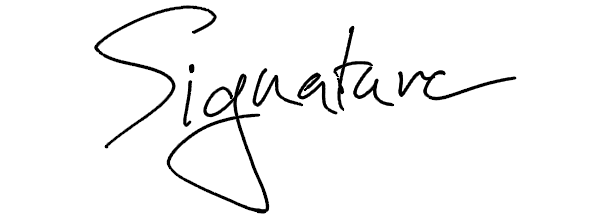
\includegraphics[width=0.3\textwidth]{img/mysignature.png}

\vspace*{-1.1cm}
\noindent \rule{0.3\textwidth}{.3pt}\\
\vspace{0.3cm}
\noindent \large{Student's name}        %%% CHANGE STUDENT'S NAME HERE


%%%%%%%%%%%%%%%%%%%%%%%%%%%%
% ABSTRACT
%%%%%%%%%%%%%%%%%%%%%%%%%%%%

\chapter*{Abstract}

\thispagestyle{empty}

\textit{\texttt{(no more than 250-300 words)}}

\subsection*{Background}
Describe background shortly

\subsection*{Aim}
Describe the aim of your study

\subsection*{Method}
Describe your methods

\subsection*{Results}
Describe the main results of your study

\subsection*{Conclusion}
State your conclusion

\subsection*{\emph{Keywords:}} No more than six keywords, preferably MeSH terms


\tableofcontents
\setcounter{page}{1}
\pagenumbering{roman}
\thispagestyle{plain}


%%%%%%%%%%%%%%%%%%%%%%%%%%%%
% LISTA DE ABREVIATURAS
%%%%%%%%%%%%%%%%%%%%%%%%%%%%

\chapter*{Lista de Abreviaturas}

%%%% En orden alfabético
\begin{itemize}
\item SDF: Signed Distance Function
\item SFI: Sistema de Funciones Iteradas
\end{itemize}
\addcontentsline{toc}{chapter}{Lista de Abreviaturas}

%%%%%%%%%%%%%%%%%%%%%%%%%%%%
% LISTA DE IMÁGENES
%%%%%%%%%%%%%%%%%%%%%%%%%%%%
\listoffigures
\thispagestyle{plain}
\addcontentsline{toc}{chapter}{Lista de Imágenes}

%%%%%%%%%%%%%%%%%%%%%%%%%%%%
% LISTA DE TABLAS
%%%%%%%%%%%%%%%%%%%%%%%%%%%%
\listoftables
\thispagestyle{plain}
\addcontentsline{toc}{chapter}{Lista de Tablas}
% \addtocontents{toc}{\bigskip}

%%%%%%%%%%%%%%%%%%%%%%%%%%%%
%%%%%%%%%%%%%%%%%%%%%%%%%%%%
% INICIO DEL TRABAJO
%%%%%%%%%%%%%%%%%%%%%%%%%%%%
%%%%%%%%%%%%%%%%%%%%%%%%%%%%

\chapter*{Introducción}
\setcounter{page}{1}
\pagenumbering{arabic}


%% TODO
TODO


\chapter{El concepto de \textit{fractal}}
\label{chap:concepto}

Las primeras preguntas que se pueden plantear son ¿qué es un fractal? ¿Qué tienen de especial estas figuras? ¿Qué las diferencia de un objeto no fractal? ¿Por qué es necesaria una geometría fractal? Trataremos de responder a cada una de estas preguntas a lo largo de este capítulo, comenzando por la primera de ellas. En realidad, hay distintas definiciones de \textit{fractal}, pero todas utilizan dos conceptos como base: la \textbf{autosimilaridad} y la \textbf{dimensión}. La primera de ellas es más cercana para nosotros de lo que en un principio podemos pensar, fijémonos en los ejemplos de la imagen \ref{fig:objetos}. 

\begin{figure}[h]
\begin{tabular}{cc}
  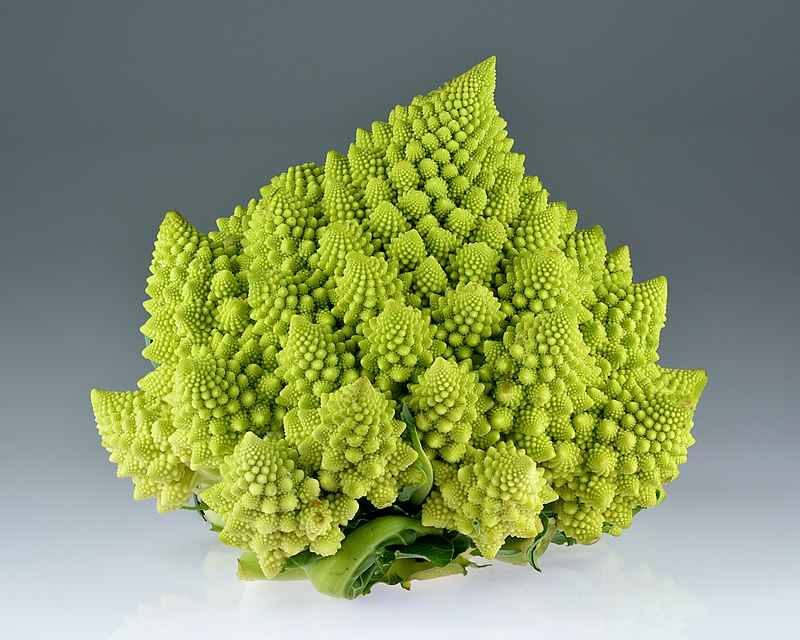
\includegraphics[scale=0.24]{./img/romanescu.jpg} &   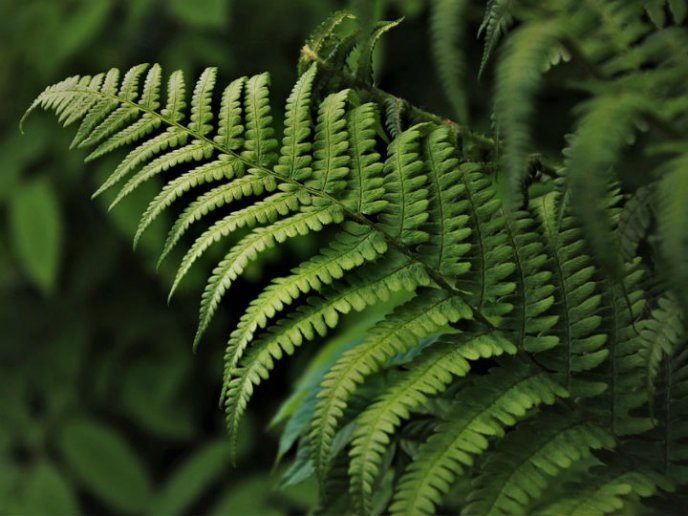
\includegraphics[scale=0.28]{./img/helecho.jpg} \\
(a) Romanescu & (b) Hoja de un helecho \\[6pt]
\end{tabular}
\caption{Objetos cotidianos con estructura fractal}
\label{fig:objetos}
\end{figure}

Observemos que el romanescu, que es un tipo de coliflor, pareciera que está formado de pequeños trozos que recuerdan el objeto original, mientras que estos pequeños trozos a su vez también están formados de pequeños trozos que recuerdan al original, y así sucesivamente. Por su parte, la hoja de un helecho también pareciera estar formada por muchas hojas más pequeñas similares a la original, y estas pequeñas hojas a su vez también están formadas por otras hojas aún más pequeñas.

Esta idea de objetos prácticamente iguales al original salvo cambios de escala es la subyacente al concepto de autosimilaridad.

\begin{definicion}[Autosimilaridad] Un objeto es \textbf{autosimilar} si está compuesto por copias de sí mismo reducidas mediante un factor de escala.
\end{definicion}

Para afianzar y formalizar conceptos y con el objetivo de introducir un concepto de dimensión, estudiaremos algunos ejemplos clásicos de objetos fractales.

\section{Ejemplos clásicos}
\label{section:ejemplos}

\subsection{El conjunto de Cantor}
\label{subsection:Cantor}

Creado por el célebre matemático \textit{George Cantor}, este fractal se construye a partir de un segmento de línea recta aplicando el siguiente proceso iterativo:

\begin{enumerate}
\item Dado el segmento de recta compuesto por el intervalo cerrado $[0,1]$, dividimos dicho segmento en tres segmentos iguales y extraemos el intervalo central, manteniendo los extremos. Es decir, extraemos el intervalo abierto $\left(\frac 1 3, \frac 2 3\right)$ y mantenemos el segmento $\left[0,\frac 1 3\right]$ y el $\left[\frac 2 3, 1\right]$. Nótese que obtenemos $2=2^0$ segmentos, cada uno a escala $\frac 1 3=\left(\frac 1 3\right)^1$ del original.

\item Aplicamos el mismo proceso a los segmentos $\left[0,\frac 1 3\right]$ y $\left[\frac 2 3, 1\right]$. Esto es, se dividen ambos en tres partes iguales y se extrae el intervalo abierto central de cada uno de ellos, manteniendo los extremos. En este caso obtendríamos $4=2^2$ segmentos iguales, cada uno de ellos a escala $\frac 1 3$ de los dos obtenidos en el primer paso y a escala $\frac 1 9=\left(\frac 1 3\right)^2$ del original.

\item Repetimos este proceso de manera indefinida, de manera que en el $n$-ésimo paso se obtendrían $2^n$ segmentos de recta a escala $\left(\frac 1 3\right)^n$.
\end{enumerate} 

Los puntos del intervalo inicial $[0,1]$ que restan tras las infinitas iteraciones son los que conforman el \textit{conjunto de Cantor}, que denotamos con $\textbf{C}$.

\begin{figure} [h]
\centering
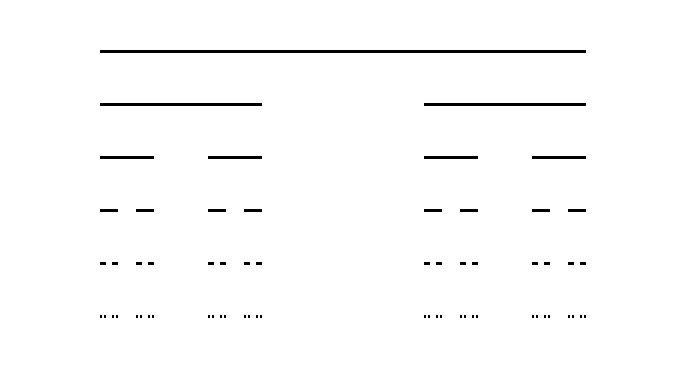
\includegraphics[scale = 0.5]{img/cantor.png}
\caption{Iteraciones del proceso de generación del conjunto de Cantor}
 \label{fig:Cantor}
\end{figure}

\subsection{La curva de Koch}
\label{subsection:curva-Koch}

Esta figura, creada por el sueco N. F. Helge von Koch sigue un proceso de construcción iterativo al igual que el conjunto de Cantor, pero en lugar de eliminar segmentos, se añaden de la siguiente manera (ver imagen \ref{fig:curva-Koch})

\begin{enumerate}
\item Partiendo de un segmento de recta de longitud $1$ (la longitud inicial es irrelevante, pues la figura final es la misma salvo un factor de escala), se divide en tres partes iguales de longitud $\frac 1 3$ y la parte central se sustituye por un triángulo equilátero al que se le elimina la base. Esto da lugar a $4=4^1$ segmentos de recta de longitud $\frac 1 3=\left(\frac 1 3\right)^1$.

\item Repetimos este proceso en cada uno de los segmentos de recta obtenidos, colocando el triángulo siempre por encima de la recta, obteniendo así $16=4^2$ segmentos de recta de longitud $\frac 1 9=\left(\frac 1 3\right)^2$.

\item Aplicamos este proceso indefinidamente, obteniendo en el paso $n$-ésimo $4^n$ segmentos de longitud $\left(\frac 1 3\right)^n$. 
\end{enumerate}

El resultado final del proceso es lo que llamamos la \textit{curva de Koch}, que denotamos como \textbf{K}

\begin{figure} [h]
\centering
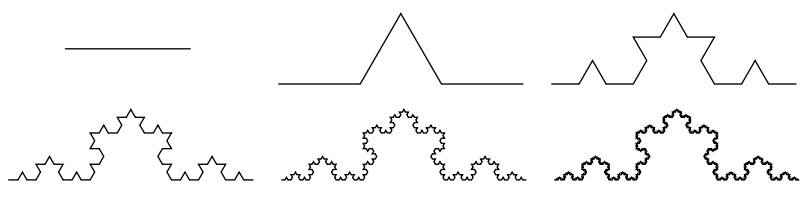
\includegraphics[scale = 0.6]{img/curva-Koch.png}
\caption{Iteraciones del proceso de generación de la curva de Koch}
 \label{fig:curva-Koch}
\end{figure}

\subsection{El copo de nieve de Koch}

A partir de la curva de Koch podemos crear un objeto matemático muy particular: el copo de nieve de Koch. Para crearlo, basta aplicar el proceso iterativo descrito para generar la curva de Koch a cada uno de los segmentos que componen un triángulo equilátero, de forma que los triángulos que se generan apunten hacia el exterior.


\begin{figure} [h]
\centering
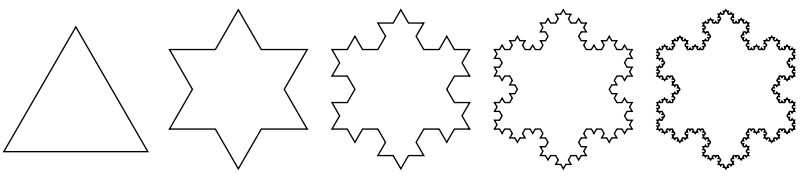
\includegraphics[scale = 0.6]{img/copo-Koch.png}
\caption{Generación del copo de nieve de Koch}
 \label{fig:copo-Koch}
\end{figure}


%%%%%%%%%%%%%%%%%%%%%%%%%%%%
% REFERENCIAS
%%%%%%%%%%%%%%%%%%%%%%%%%%%%

\bibliographystyle{agsm}
\bibliography{references}
% \addtocontents{toc}{\bigskip}
\addcontentsline{toc}{part}{Bibliography}


%%%%%%%%%%%%%%%%%%%%%%%%%%%%
% APENDICES
%%%%%%%%%%%%%%%%%%%%%%%%%%%%

\appendix
\cleardoublepage
% \addtocontents{toc}{\bigskip}
\addcontentsline{toc}{part}{Appendices}

%% OPTIONAL - Max 10-15 pages in total

\chapter{Appendix title}

\chapter{Another Appendix}

\end{document}